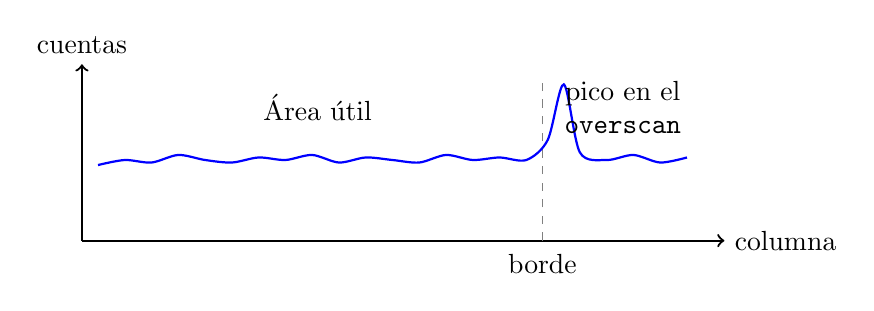
\begin{tikzpicture}[x=0.68cm,y=0.32cm]
  \draw[->,thick] (0,0) -- (12,0) node[right] {columna};
  \draw[->,thick] (0,0) -- (0,7) node[above] {cuentas};
  \draw[gray,dashed] (8.6,0) -- (8.6,6.4);
  \draw[blue,thick,smooth] plot coordinates {
    (0.3,3.0) (0.8,3.2) (1.3,3.1) (1.8,3.4) (2.3,3.2)
    (2.8,3.1) (3.3,3.3) (3.8,3.2) (4.3,3.4) (4.8,3.1)
    (5.3,3.3) (5.8,3.2) (6.3,3.1) (6.8,3.4) (7.3,3.2)
    (7.8,3.3) (8.3,3.2) (8.7,4.0) (9.0,6.2) (9.3,3.5)
    (9.8,3.2) (10.3,3.4) (10.8,3.1) (11.3,3.3)
  };
  \node[align=center] at (4.4,5.3) {Área útil};
  \node[align=center] at (10.1,5.3) {pico en el\\\texttt{overscan}};
  \node[below] at (8.6,-0.15) {borde};
\end{tikzpicture}